\section{STRUCTURE, ORGANIZATION, AND IMPLEMENTATION}

	\subsection{CATEGORIES OF LIFE CYCLE PROCESSES}

	\begin{figure}[h]
		\centering
		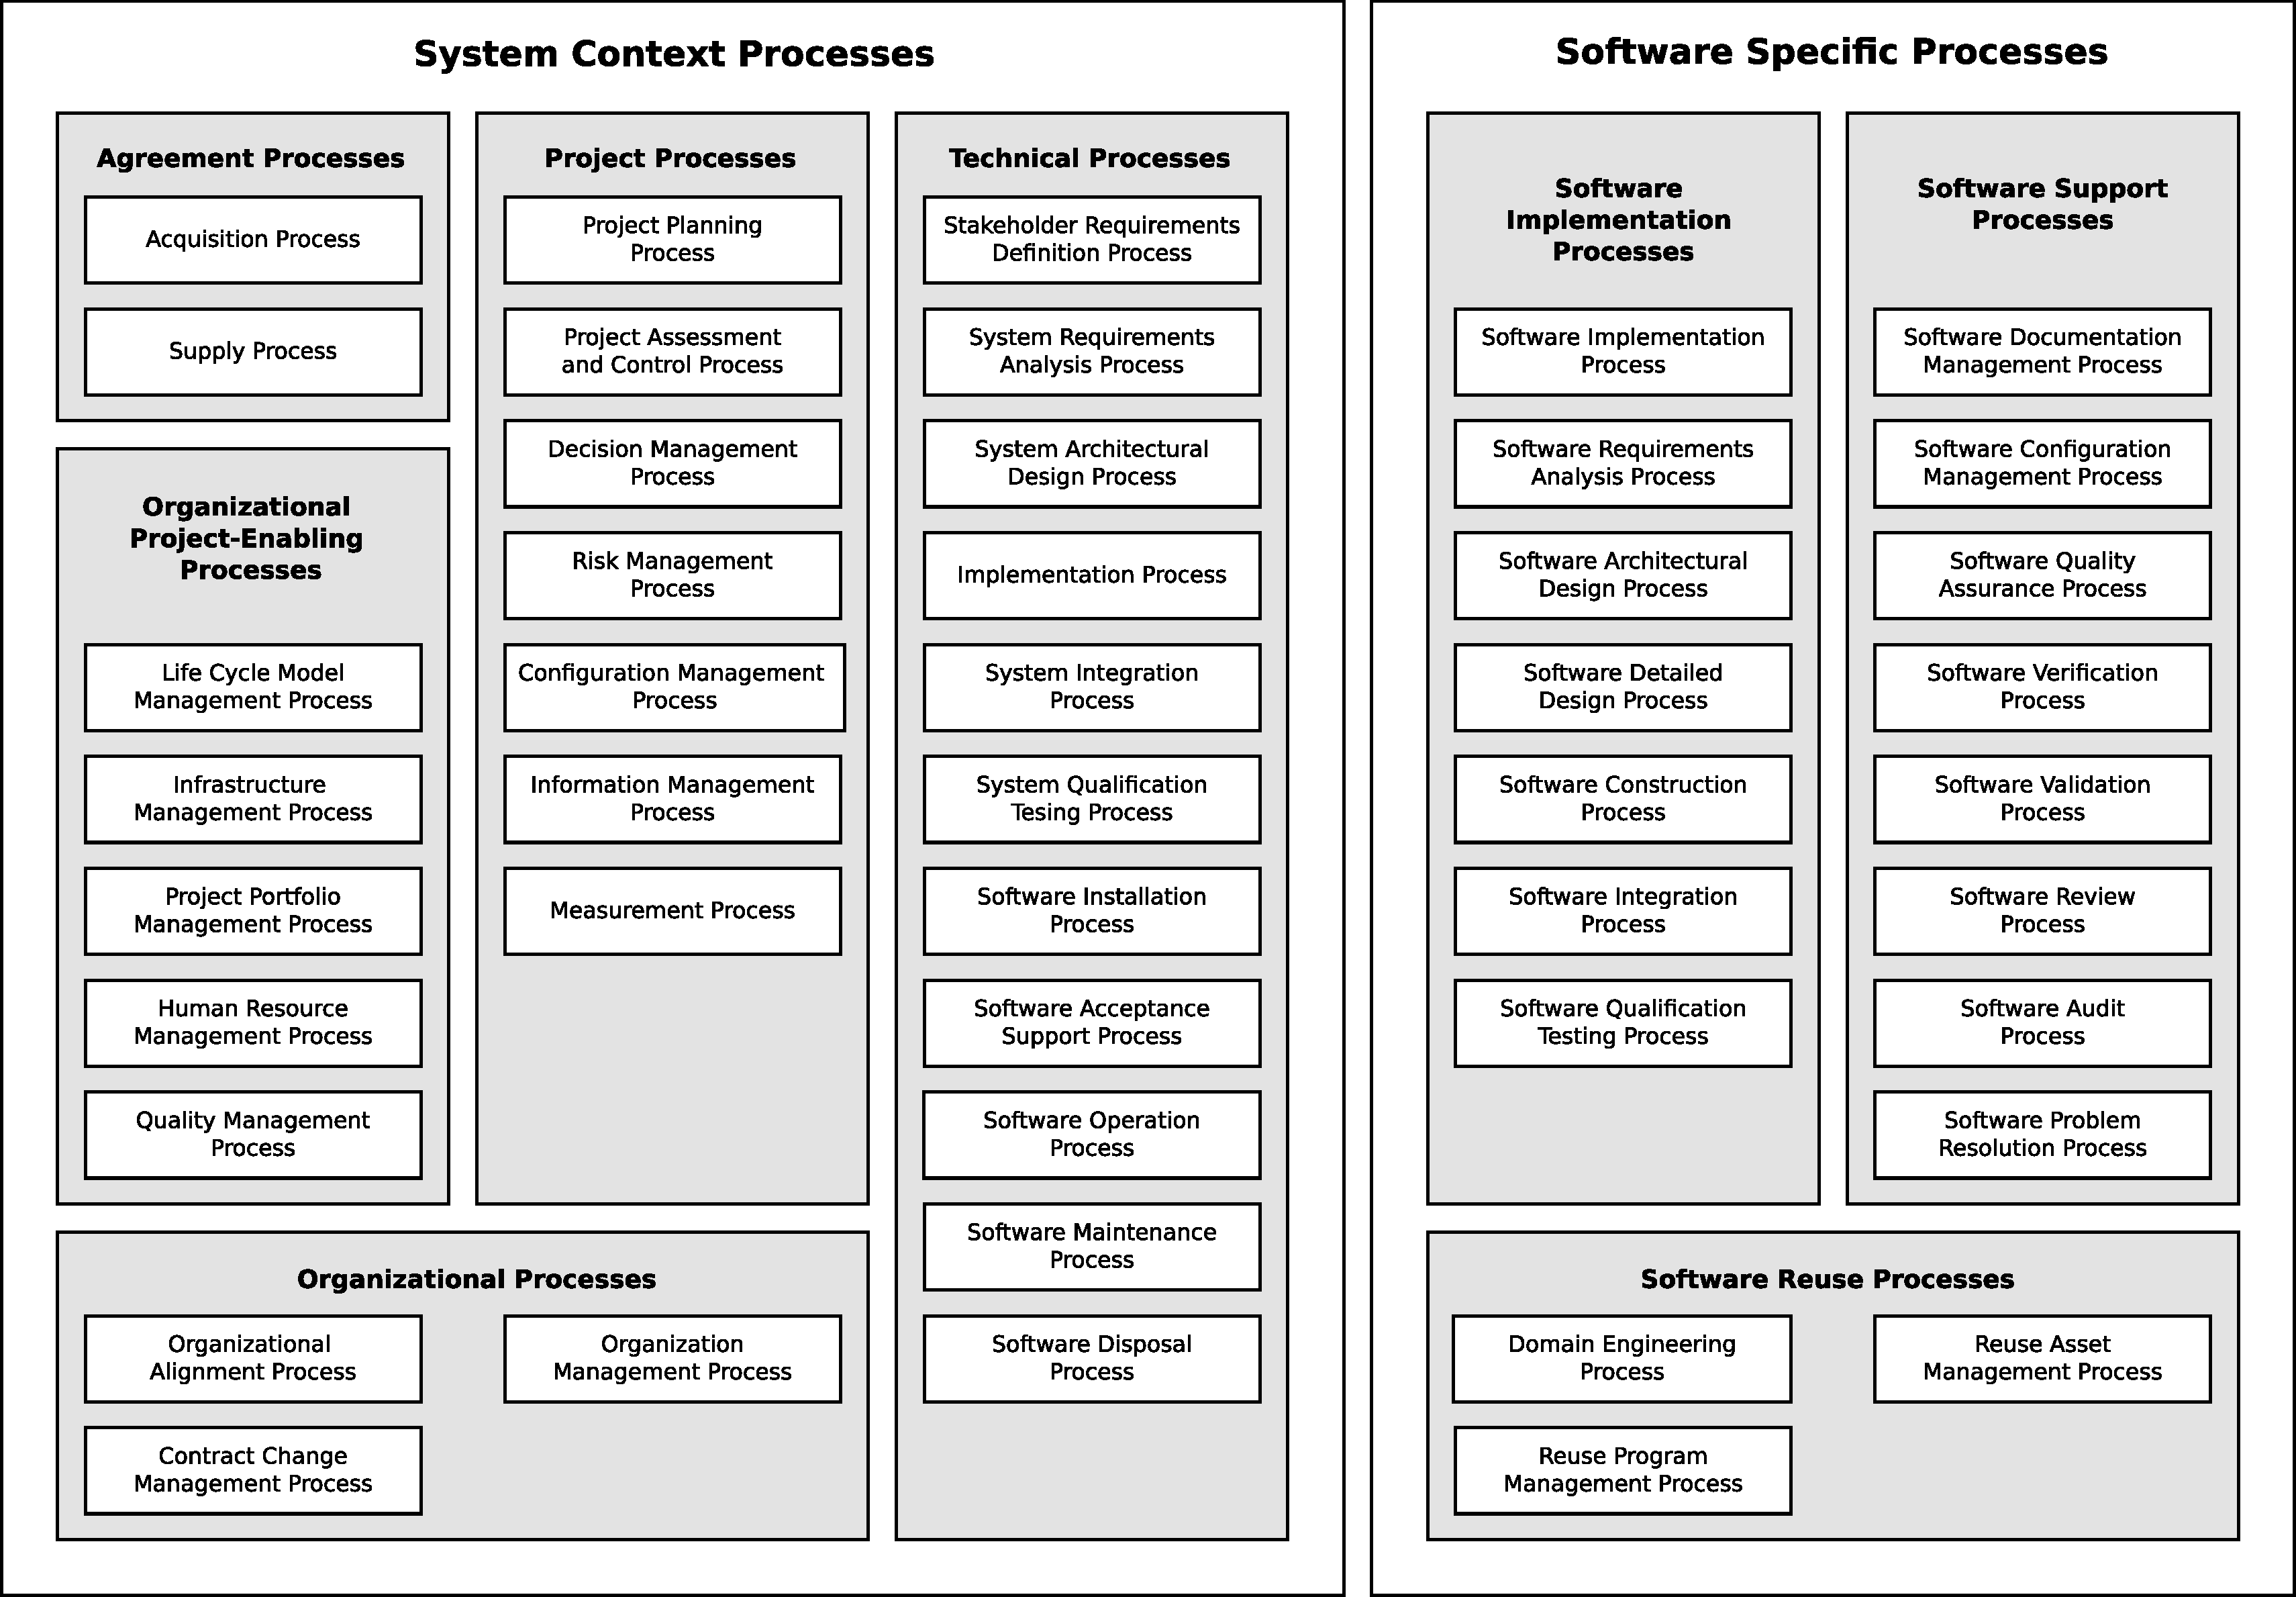
\includegraphics[width=17cm,keepaspectratio]{figures/life-cycle-process-groups.pdf}
		\caption{Process Reference Model (PRM)}
		\label{fig:life_cycle_process_groups}
	\end{figure}

	\begin{adjustwidth}{0.5em}{0pt}

		To facilitate practical understanding and application of this standard, we have grouped the activities that may be performed during the life cycle of a software system into seven process groups. Each of the life cycle processes within those groups is described in terms of its purpose and desired outcomes, and lists activities and tasks which need to be performed to achieve those outcomes.

		The purpose and outcomes of the life cycle processes constitute a Process Reference Model (PRM), where each process group is contained within its own distinct section, the process groups and their processes are sub-sections within those sections, and each sub-section / process contains sub-sub-sections for their purpose, outcome, activities, and tasks. 

	\end{adjustwidth}

	\subsection{SUMMARY OF LIFE CYCLE PROCESSES}
	\begin{adjustwidth}{0.5em}{0pt}

		There are two major sub-divisions of process within this standard, where Section \nameref{sec:system_context_processes} provides a system context for dealing with a standalone software product or service of a software system, and Section \nameref{sec:software_specific_processes} contains the software-specific processes for use in implementing a software product or service that is an element of a larger system. Brief summarization of these divisions' process groups may be found below.

	\end{adjustwidth}

		\subsubsection{AGREEMENT PROCESSES}
		\begin{adjustwidth}{1em}{0pt}

			\nameref{subsec:agreement_processes} define the activities necessary to establish an agreement between two organizations. 

		\end{adjustwidth}

		\subsubsection{ORGANIZATIONAL PROJECT-ENABLING PROCESSES}
		\begin{adjustwidth}{1em}{0pt}

			The \nameref{subsec:organizational_project_enabling_processes} manage the organization's capability to acquire and supply products or services through the initiation, support and control of projects. They provide resources and infrastructure necessary to support projects and ensure the satisfaction of organizational objectives and established agreements.

		\end{adjustwidth}

		\subsubsection{PROJECT PROCESSES}
		\begin{adjustwidth}{1em}{0pt}

			There are two categories of \nameref{subsec:project_processes}. The Project Management Processes are used to plan, execute, assess and control the progress of a project. The Project Support Processes support specialized management objectives.

		\end{adjustwidth}

		\subsubsection{ORGANIZATIONAL PROCESSES}
		\begin{adjustwidth}{1em}{0pt}

			The \nameref{subsec:organizational_processes} are highly useful, in that they help organizations ensure their processes are aligned and consistent with its business goals.

		\end{adjustwidth}

		\subsubsection{TECHNICAL PROCESSES}
		\begin{adjustwidth}{1em}{0pt}

			The \nameref{subsec:technical_processes} are used to define the requirements for a system, to transform the requirements into an effective product, to permit consistent reproduction of the product where necessary, to use the product, to provide the required services, to sustain the provision of those services and to dispose of the product when it is retired from service.

		\end{adjustwidth}

		\subsubsection{SOFTWARE IMPLEMENTATION PROCESSES}
		\begin{adjustwidth}{1em}{0pt}

			The \nameref{subsec:software_implementation_processes} are used to produce a specified system element (software item) implemented in software. 

			Those processes transform specified behavior, interfaces and implementation constraints into implementation actions resulting in a system element that satisfies the requirements derived from the system requirements.

		\end{adjustwidth}

		\subsubsection{SOFTWARE SUPPORT PROCESSES}
		\begin{adjustwidth}{1em}{0pt}

			The \nameref{subsec:software_support_processes} provide a specific focused set of activities for performing a specialized software process. A supporting process assists the Software Implementation Process as an integral part with a distinct purpose, contributing to the success and quality of the software project.

		\end{adjustwidth}

		\subsubsection{SOFTWARE REUSE PROCESSES}
		\begin{adjustwidth}{1em}{0pt}

			The \nameref{subsec:software_reuse_processes} consists of three processes that support an organization's ability to reuse software items across project boundaries. These processes are unique because, by their nature, they operate outside the bounds of any particular project.

		\end{adjustwidth}


	\subsection{STANDARD AS PROCESS REFERENCE MODEL (PRM)}
	\begin{adjustwidth}{0.5em}{0pt}

		A Process Reference Model (PRM) provides a level of abstraction higher than that of the detailed required contained with any given standard or specification, and is applicable to an organization that is assessing its processes in order to determine their own capabilities and limitations. 
		
		A Process Reference Model, by definition, must contain the following:

		\begin{compactenum}

			\item A declaration of the target domain

			\item A description of the processes within its scope

			\item A description of the relationship between itself and its intended context of use

			\item A description of the relationship between the processes defined within itself

		\end{compactenum}


		A Process Reference Model does not necessarily represent a particular process implementation approach, nor does it prescribe a system/software life cycle model, methodology, or technique. Instead, the reference model is intended to be adopted by an organization based on its business needs and application domain. 

		Furthermore, the organization's defined process is adopted by the organization's projects in the context of the projects' requirements. 

		In order to ensure this standard serves as a legitimate Process Reference Model, it has been written and structured in a manner and method that satisfies international standards and guidelines while also, hopefully, being informative, educational, and useful to its readers. 

	\end{adjustwidth}